\chapter{Résultats}\label{resultats}

Ce chapitre présente les résultats des principales expérimentations réalisées, généralement sous forme de couple d'entraînements. Sauf indications contraires (scores en italique), les précision et recall mentionnés sont issus de l'évaluation du modèle sur le dataset de test constitué en début de stage (5918 images).

\section{Tests}

Pour vérifier notre méthode, il m'a été demandé d'entraîner le modèle sur le même dataset que celui utilisé
dans l'article, pour comparer les résultats. Nous avons évalué les deux modèles sur la partie du dataset
COCO validation 2017 (121 images, 1201 détections) qui est constituée uniquement des images
contenant des bateaux.
Bien que les deux modèles n'aient pas étés entraînés de la même façon (300 époques pour le modèle téléchargé,
30 pour celui que nous avons entraîné), nous avons obtenu des résultats très proches :

\begin{table}[!h]
    \caption{YOLOX entraîné par notre équipe comparé à YOLOX entraîné par les auteurs.}
\begin{center}
    \begin{tabular}{ c c c }
        \hline
        & YOLOX-S entraîné & YOLOX-S téléchargé \\
        \hline
        mAP & 24.326 & 25.361 \\
        mAR & 45.118 & 43.585
    \end{tabular}
\end{center}
\end{table}

On peut donc en conclure que notre entraînement est efficace.

Nous avons par la suite testé sur de petits datasets, puis documenté,
l'effet de différents hyper-paramètres :

\begin{itemize}
    \item \texttt{input\_size} : définit la taille du tenseur (correspondant à l'image) accepté en entrée du modèle ;
    \item \texttt{n\_batch} : définit le nombre d'images utilisé à chaque itération au sein d'une époque.
    \item \texttt{random\_size} : paramètre de data augmentation ;
    \item \texttt{multiscale\_range} : paramètre de data augmentation.
\end{itemize}

Ces essais ont été très utiles, car ils nous ont permis de déterminer la taille de batch
optimale \cite{Goodfellow-et-al-2016} pour chaque machine avec différentes cartes graphiques :
7 pour la RTX 4070 Ti Super et 3 pour la RTX 4060.
Les tailles de batch sont proportionnelles à la taille de la mémoire graphique
disponible sur chaque carte. Une taille de batch trop petite demanderait de diminuer le "learning rate"
\footnote{Le "learning rate" détermine la vitesse à laquelle le réseau peut adapter ses poids
pour apprendre des exemples qui lui sont fournis.}, et une taille de batch trop grande
saturerai la mémoire vidéo, ce qui impliquerait d'utiliser la mémoire classique de l'ordinateur.
Cette dernière situation n'est pas souhaitable, car elle multiplie par plusieurs dizaines
le temps d'entraînement (la mémoire était bien plus lente que la mémoire vidéo).

Enfin, à la demande de notre maître de stage, nous avons comparé deux entraînements pour évaluer
l'effet de l'index du label sur les performances.
En effet, les modèles utilisés sont pré-entraînés avec 80 classes, la huitième correspondant
au label "boat". Le premier entraînement a été effectué avec le label boat et son index d'origine,
le second a été fait avec le label boat à l'index 0.
Pendant les cinq première époques, le premier avait des performances plus élevée (évaluation sur
le dataset de validation), mais aucune différence ne subsistait à la fin de l'entraînement.
On peut supposer que les poids d'origine ont une influence au début de l'entraînement.


\section{Tuilage}

D'après nos recherches, le tuilage est un moyen efficace d'augmenter les performances d'un modèle après
entraînement. Il consiste à diviser l'image en plusieurs parties, afin d'éviter d'avoir à la compresser
(et donc perdre en résolution).
YOLOX contient des couches de convolution\footnote{La convolution est un opérateur mathématique
qui permet de mettre en correspondance des signaux spatiaux avec un filtre ou un noyau,
pour détecter des patterns ou des caractéristiques spécifiques.}, et, selon notre raisonnement,
un objet trop petit (contenant peu de pixels) risque d'être effacé par ces couches, et n'apporter
aucune information utile à l'apprentissage du modèle.
Afin de tester notre hypothèse, avons tenté d'appliquer le tuilage avant l'entraînement,
et ainsi de réduire le nombre de petits objets dans le dataset.
Nous avons pour cela utilisé SAHI \cite{Akyon_Altinuc_Temizel_2022}.

Nous avons fait trois expérimentations comprenant deux entraînements chacune.
Les datasets d'entraînement contenait uniquement 1000 images, tirées au hasard parmi tous les datasets,
afin de connaître rapidement le résultat.

Pour chaque expérimentation, un des entraînements était fait sur des tuiles de 640 pixels de côté,
provenant des images originales.

Voici les précisions et rappels mesurés sur le dataset de test :\\

\begin{table}[h]
    \begin{center}
        \begin{tabular}{c c c}
            \hline
            & Images tuilées & Images originales \\
            \hline
            mAP & 34.001 & 35.276 \\
            mAR & 50.249 & 50.654 \\
        \end{tabular}
    \end{center}
    \caption{Tuilage pré-entraînement, 3 tests avec petits datasets (moyenne des résultats).}
\end{table}

Le tuilage pré-entraînement a un impact sensiblement négatif sur les performances du modèle.

À la demande de notre maître de stage, nous avons réitéré cette expérimentation sur un
dataset plus conséquent, composé de toutes les images à notre disposition, filtrées
avec les seuils de similarité que nous avons déterminé. Ceci représente
30 000 images.

\begin{table}[h]
    \begin{center}
        \begin{tabular}{c c c}
            \hline
            & Images tuilées & Images originales \\
            \hline
            mAP & 55.003 & 60.536 \\
            mAR & 63.896 & 67.477 \\
        \end{tabular}
    \end{center}
    \caption{Tuilage pré-entraînement.}
\end{table}

La conclusion est similaire aux entraînements de test effectués précédemment :
le tuilage avant entraînement réduit de manière significative la précision et
le rappel du modèle.

\section{Images vides}

Ces entraînements ont pour but de déterminer si la présence d'images sans bateaux pendant l'entraînement
permet de réduire le nombre de faux positifs durant l'inférence.

Pour créer un dataset contenant des images vides, nous avons utilisé le tuilage, car SAHI permet
de facilement conserver ou non les tuiles issues de parties d'image sans détections.

Voici les résultats obtenus avec 3000 images (avant tuilage) : \\

\begin{table}[h]
    \begin{center}
        \begin{tabular}{c c c}
            \hline
            & Tuilage simple & Tuilage avec suppression des tuiles vides \\
            \hline
            mAP & 43.875 & 43.765 \\
            mAR & 56.028 & 55.201 \\
        \end{tabular}
    \end{center}
    \caption{Tuilage avec ou sans conservation des images vides.}
\end{table}

Nous tirons comme conlusion de cet entraînement qu'ajouter des images videss
n'a pas d'impact sur les performances du modèle.

\section{Scinder la classe boat}

Ces entraînements ont pour but de savoir si diviser les bateaux en plusieurs
catégories améliore la précision générale du modèle.
Les entraînements ont été fait sur le dataset \texttt{ABOships-PLUS},
car il contient les classes "powerboat", "sailboat" et "ship"
et un nombre d'images suffisant (5866 images).

Le dataset de test constitué au début du stage ne permet pas l'évaluation du modèle, car les différentes classes utilisées pendant l'entraînement ne sont pas présentes.
Nous avons donc retenu les résultats issus de l'évaluation sur le dataset de validation
à la dernière époque, puis nous avons calculé une moyenne pondérée des précision
et rappels pour les classes powerboat, sailboat et ship. \\

\begin{table}[h]
    \begin{center}
        \begin{tabular}{c c c}
            \hline
            & Classe unique & Classes multiples (moyenne) \\
            \hline
            
            \textit{mAP} & 41.828 & 40.856 \\
            \textit{mAR} & 53.520 & 53.475 \\
            
        \end{tabular}
    \end{center}
    \caption{Entraînement avec plusieurs classes.}
\end{table}

On observe une légère diminution de la précision et du rappel lorsqu'on tente de prédire plusieurs
classes. \\

Pour aller plus loin, nous avons créé une seconde expérimentation, cette fois-ci à partir
de trois datasets différents : \texttt{dataset\_GLSD}, \texttt{SMD\_plus}, \texttt{vessel\_detection\_v21}.
Nous avons choisi ces derniers car ils comportaient des classes similaires que nous avons pu réunir :
"cargo", "ferry", "sailing boat", "fishing boat". \\

\begin{table}[H]
    \begin{center}
        \begin{tabular}{c c c c c c}
            \hline
            & cargo & ferry & fishing boat & sailing boat & \textbf{moyenne} \\
            \hline
            
            \textit{mAP} & 53.895 & 88.126 & 67.593 & 73.628 & \textbf{71.923}\\
            \textit{mAR} & 59.922 & 90.230 & 71.718 & 76.653 & \textbf{75.692}\\
                % }
        \end{tabular}
    \end{center}
    \caption{Entraînement avec plusieurs classes (3 datasets).}
\end{table}

La moyenne ci-dessus a été pondérée par le nombre de bateaux dans chaque classe. 

\begin{table}[H]
    \begin{center}
        \begin{tabular}{c c}
            \hline
            & boat  \\
            \hline

            \textit{mAP} & 75.859 \\
            \textit{mAR} & 78.416 \\
                % }
        \end{tabular}
    \end{center}
    \caption{Entraînement avec une classe (3 datasets).}
\end{table}

On observe encore une fois une diminution de la précision au profit de la capacité à classifier
les bateaux.

Nous concluons des résultats précédents que diviser les bateaux en plusieurs classes plus précises
ne permet par d'améliorer les scores globaux lors de l'évaluation du modèle. Cependant,
l'intérêt du point de vue commercial est indéniable. Nous avons donc entrepris de faire des
entraînements à partir de datasets annotés par nos soins, selon une liste de classes
la plus précise possible (\textit{voir annexe \ref{classes_annotations}}).\\

Les scores du modèle en fonction des classes sont les suivants : \\

\begin{table}[H]
    \begin{center}
        \begin{tabular}{c c c c c c c c c}
            \hline
            boat & breakwater & bulker & buoy & cargo & cruise & ferry & fishing \\
            \hline
            
            \textit{mAP} & 39.839 & 44.762 & 79.066 & 42.374 & 79.203 & 90.311 & 81.185 & 72.556 \\
            \textit{mAR} & 54.493 & 58.744 & 85.000 & 49.788 & 82.153 & 92.163 & 85.623 & 77.036 \\
                % }
            \hline
            lighthouse & luxury & platform & recreational & sailboat & service & warship & \textbf{moyenne} \\
            \hline
            
            \textit{mAP} & 50.190 & 80.628 & 33.638 & 60.410 & 60.314 & 53.784 & 85.930 & \textbf{66.532 }\\
            \textit{mAR} & 57.046 & 84.431 & 68.276 & 67.511 & 67.125 & 64.032 & 88.831 & \textbf{73.235 }\\
        \end{tabular}
    \end{center}
    \caption{Entraînement avec plusieurs classes (3 datasets).}
\end{table}

On remarque que certaines classes sont plus difficiles à prédire que d'autres.
Puisque nous connaissons la précision du modèle pour chaque classe, nous avons suggéré d'adapter les
seuils de confiance (appliqués lors de l'inférence) en fonction de la précision de chaque classe.
Par exemple, la classe "platform" étant la plus difficile à prédire, on appliquerait un seuil plus élevé afin
que seules les détections avec une confiance très élevée soient affichées.

Cependant, en conduisant des analyses plus poussées, ceci ne semble pas être une bonne solution. Nous avons supposé que les classes obtenant le plus faible rappel sont celles qui contiennent les objets les plus lointains ou difficiles à détecter.
Le score de corrélation  (Pearson) entre la taille des détections et la précision est de 0.60025, donc peu significatif. Malgré une faible corrélation, il faut faire attention à ne pas confondre les classes
difficiles à prédire et les classes ne contenant que des petits objets.

\begin{figure}[H]
    \centering
    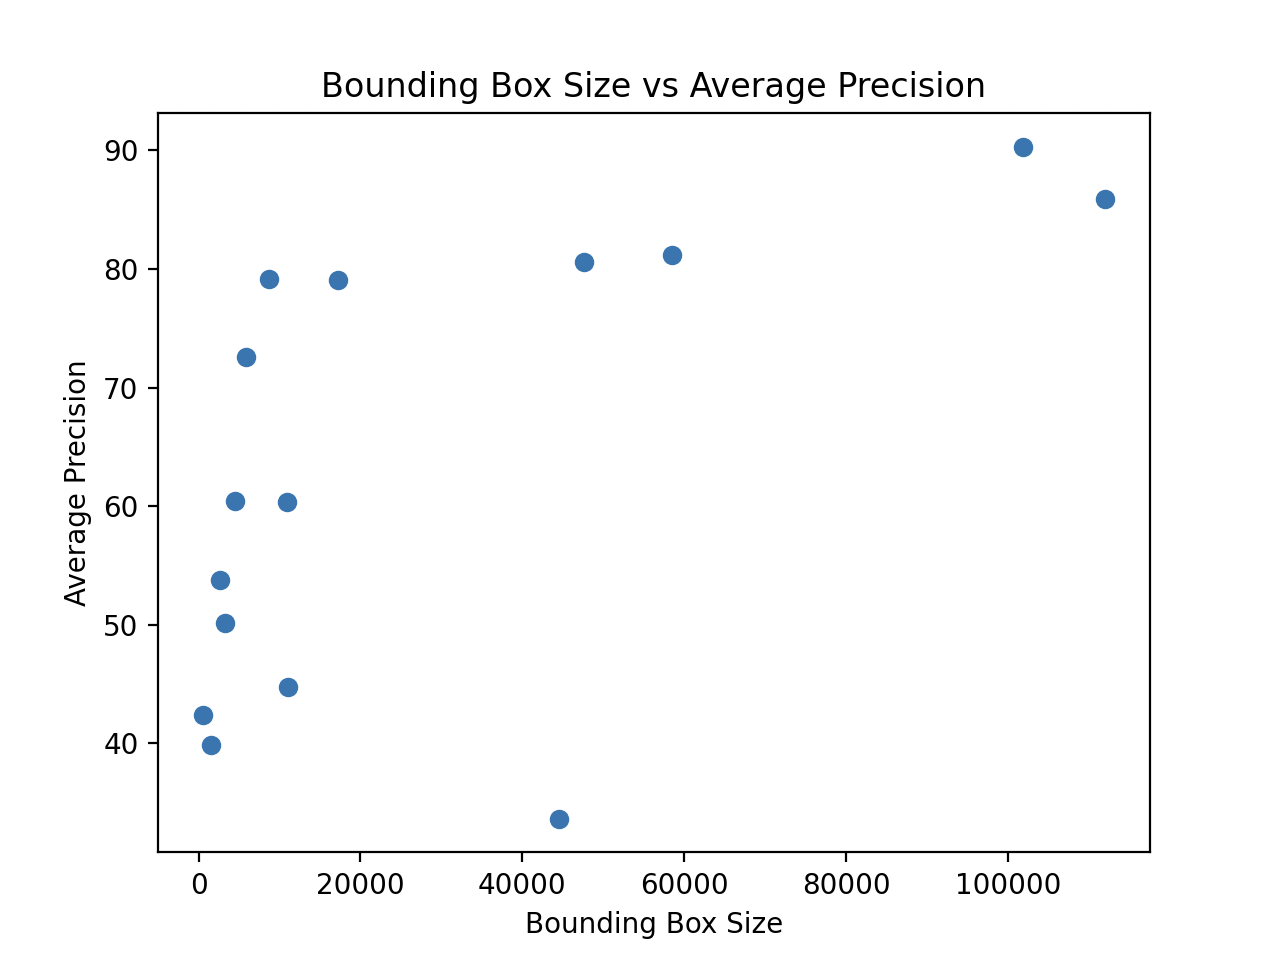
\includegraphics[width=0.45\textwidth]{./img/size_precision.png}
    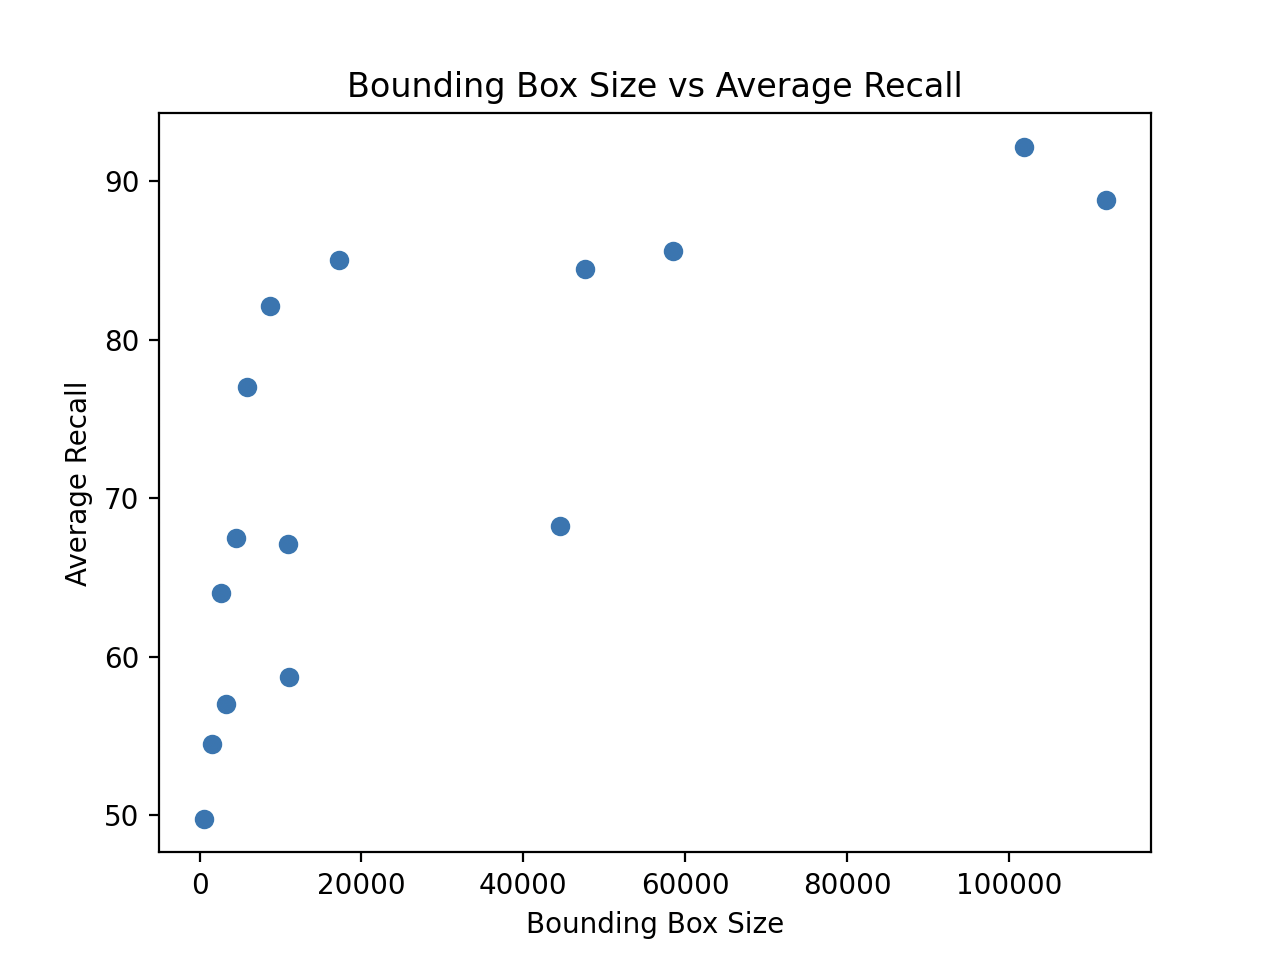
\includegraphics[width=0.45\textwidth]{./img/size_recall.png}
    \caption{Précision et rappel en fonction de la taille des objets.}
\end{figure}

\section{Images faciles à identifier}

Nos expériences nous ont conduit à nous demander si des images plus faciles à identifier, c'est-à-dire
en haute définition, contrastées et lumineuses, permettait au réseau de neurones de mieux apprendre les
traits caractéristiques des bateaux, et donc d'obtenir de meilleurs scores.

Pour répondre à cette question, nous avons utilisé le dataset \texttt{marvel} dont les bateaux occupaient
toutes l'image et étaient en général situés au centre. Le nombre d'images était de 11502 pour cet entraînement. \\

\begin{table}[H]
    \begin{center}
        \begin{tabular}{c c c}
            \hline
            & marvel & images tirées au hasard\\
            \hline
            mAP & \textit{19.252} & 47.858 \\
            mAR & \textit{27.436} & 57.285 \\
        \end{tabular}
    \end{center}
    \caption{Entraînement avec image facile à identifier.}
\end{table}

Ces scores montrent qu'il vaut mieux entraîner YOLOX avec des images représentatives de
l'environnement d'inférence.

\section{Résultats précédents}

Le modèle entraîné l'année dernière a été évalué sur note dataset de test : \\

\begin{table}[h]
    \begin{center}
        \begin{tabular}{c c c c}
            \hline
            & YOLOX-S base & Meilleur modèle 2023 & \textbf{Meilleur modèle 2024} \\
            \hline
            mAP & 25.361 & 32.903 & 60.907 \\
            mAR & 43.585 & 47.276 & 66.471 \\
        \end{tabular}
    \end{center}
    \caption{Comparaison avec notre meilleur modèle.}
\end{table}

Ce tableau montre les progrès que nous avons fait dans la détéction de navires,
et permettent de valider l'efficacité de nos travaux durant le stage.
